\documentclass[12pt,]{article}
\usepackage[left=1in,top=1in,right=1in,bottom=1in]{geometry}
\newcommand*{\authorfont}{\fontfamily{bch}\selectfont}
\usepackage{lmodern}
\usepackage{abstract}
\renewcommand{\abstractname}{}    % clear the title
\renewcommand{\absnamepos}{empty} % originally center

\renewenvironment{abstract}
 {{%
    \setlength{\leftmargin}{0mm}
    \setlength{\rightmargin}{\leftmargin}%
    \footnotesize
  }%
  \relax}
 {\endlist}

\makeatletter
\def\@maketitle{%
  \newpage
%  \null
  \let \footnote \thanks
    {\fontsize{18}{20}\selectfont\centering  \setlength{\parindent}{0pt} \@title \par}%
  \vskip 2em%
}
%\fi
\makeatother




\setcounter{secnumdepth}{0}



\title{Why are More Trade-Open Countries More Likely to Repress the Media? }



\author{}


\date{}

\usepackage{titlesec}

\titleformat*{\section}{\normalsize\bfseries}
\titleformat*{\subsection}{\normalsize\itshape}
\titleformat*{\subsubsection}{\normalsize\itshape}
\titleformat*{\paragraph}{\normalsize\itshape}
\titleformat*{\subparagraph}{\normalsize\itshape}

\usepackage{natbib}
\bibliographystyle{plainnat}


\newtheorem{hypothesis}{Hypothesis}
\usepackage{setspace}

\makeatletter
\@ifpackageloaded{hyperref}{}{%
\ifxetex
  \usepackage[setpagesize=false, % page size defined by xetex
              unicode=false, % unicode breaks when used with xetex
              xetex]{hyperref}
\else
  \usepackage[unicode=true]{hyperref}
\fi
}
\@ifpackageloaded{color}{
    \PassOptionsToPackage{usenames,dvipsnames}{color}
}{%
    \usepackage[usenames,dvipsnames]{color}
}
\makeatother
\hypersetup{breaklinks=true,
            bookmarks=true,
            pdfauthor={},
            pdfkeywords = {},  
            pdftitle={Why are More Trade-Open Countries More Likely to Repress the Media?},
            colorlinks=true,
            citecolor=MidnightBlue,
            urlcolor=MidnightBlue,
            linkcolor=MidnightBlue,
            pdfborder={0 0 0}}
\urlstyle{same}  % don't use monospace font for urls

\begin{document}  

% \maketitle

{% \usefont{T1}{pnc}{m}{n}
\setlength{\parindent}{0pt}
\thispagestyle{plain}
{\fontsize{18}{20}\selectfont\centering
\maketitle  % title \par  

}

{
   \relax \centering \normalsize\fontsize{11}{12} 

  \vskip 1.5em%
}

}





\vskip 6.5pt

\noindent \doublespacing Given the conventional wisdom that democratic political institutions
drive economic openness @{[}Milner:2005ci{]} and vice-versa
@{[}EICHENGREEN:2008gg{]}, it is surprising that since the 1970s, on
average, those countries which have been more open to international
trade have had lower levels of media freedom. Although overall economic
globalization is positively correlated with media freedom around the
world, the bivariate relationship between trade and media freedom is
weakly negative. The bottom half of Figure 1 shows that for all
available country-years between 1970 and 2011, those which engaged in
higher levels of international trade had slightly more repressive media,
on average, than those countries which were less open to international
trade. This is true in both historically democratic and non-democratic
countries, although the difference is most clear among countries with
more democratic histories. Given the positive correlation found between
media freedom and economic globalization as measured by the KOF index
for overall economic globalization @{[}Dreher:2008dg{]}, the coincidence
of higher trade openness and greater media repression is a surprisingly
under-reported empirical puzzle in international and comparative
political economy.

\begin{center}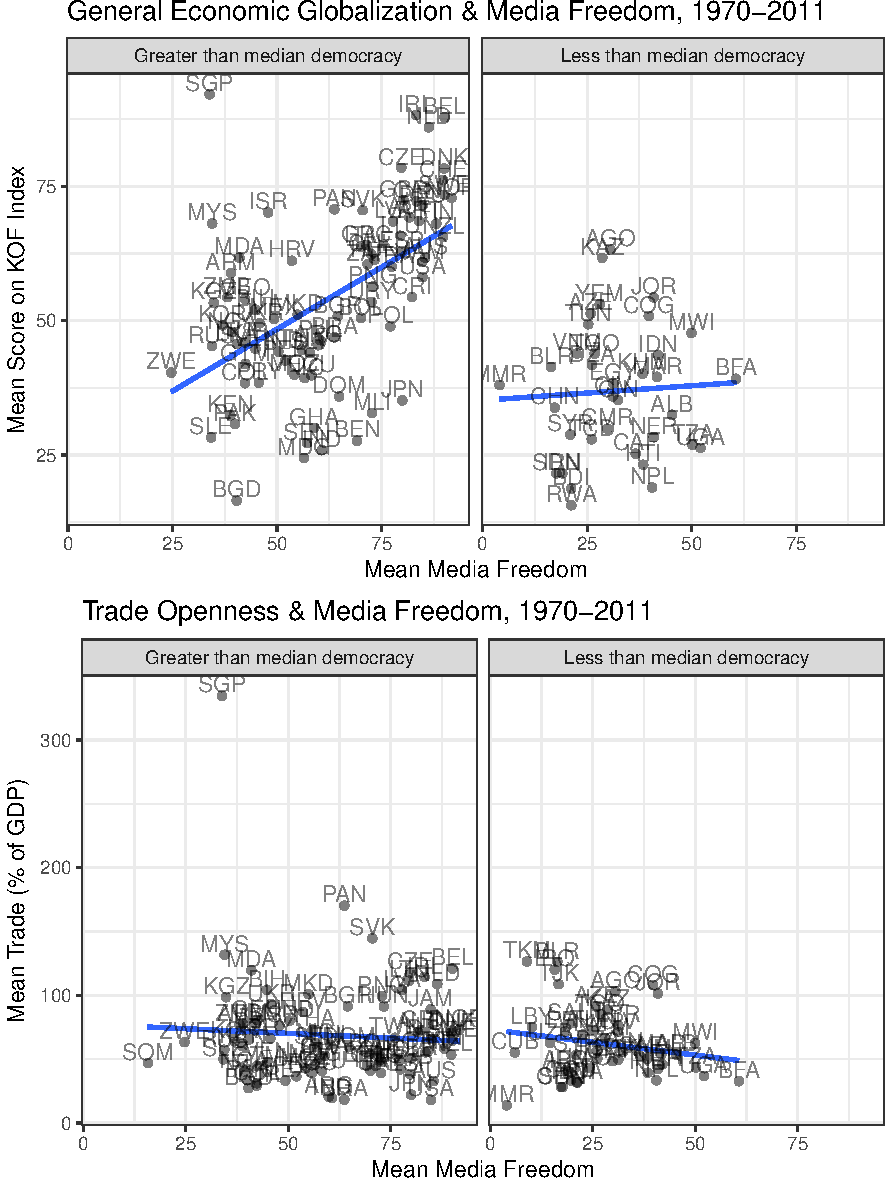
\includegraphics[width=0.8\linewidth]{figures/unnamed-chunk-1-1} \end{center}

\newpage

\bibliography{mybib}

\end{document}
